% This is based on the LLNCS.DEM the demonstration file of
% the LaTeX macro package from Springer-Verlag
% for Lecture Notes in Computer Science,
% version 2.4 for LaTeX2e as of 16. April 2010
%
% See http://www.springer.com/computer/lncs/lncs+authors?SGWID=0-40209-0-0-0
% for the full guidelines.
%
\documentclass{llncs}
\usepackage{graphicx}
\begin{document}

\title{Learning Probabilistic Models for Object Location }
%
\titlerunning{Hamiltonian Mechanics}  % abbreviated title (for running head)
%                                     also used for the TOC unless
%                                     \toctitle is used
%
\author{Deebul Nair\inst{1} \and Tim Niemueller \inst{2}
\and Gerhard Pl\"{o}ger \inst{1} \and Gerhard Lakemeyer \inst{2}}
%
\authorrunning{Deebul Nair et al.} % abbreviated author list (for running head)
%
%
\institute{Bonn-Rhein-Sieg University of Applied Sciences\\Department of Computer Science\\ 
Sankt Augustin, Germany\\
\email{{<deebul.nair, paul.ploeger>}@inf.h-brs.de},
\and
Knowledge-based Systems Group\\
RWTH Aachen University, Aachen, Germany \\
\email{{<niemueller, gerhard>}@kbsg.rwth-aachen.de}}
\maketitle              % typeset the title of the contribution

\begin{abstract}
In this paper our aim is to predict locations of objects in a particular home environment, where the robot has the map of the environment and the knowledge of previous locations of the objects . We argue that by making use of temporal information for prediction improves the prediction of the location of an object. To realize this, we develop a probabilistic models to capture the dynamics of observed objects, called as the object location model. The object location model will make use of both spatial and temporal information recorded by the robot to make predictions. Even though all homes show much similarity in their spatial organization, the usage of the space and the objects in it is entirely based on the user’s preferences. Most of the previous work on object location prediction is based upon predicting the object’s location in a generic home while the proposed model will make predictions for a specific home. We demonstrate the validity of the approach by comparing it with the state of the art prediction algorithm. 
\keywords{Probabilistic Models, Spatio-Temporal learning}
\end{abstract}
%
\section{Introduction}
As robots move from more structured environments of laboratories to unstructured environments like homes and offices, multiple challenges arises. One of the challenge is
estimating the location of objects in less structured and more uncertain environments.
This challenge led to probabilistic mapping of objects location in the environment, which
enables estimating objects location based on last seen information. Some authors have
made effort to obtain information about the world dynamics and proposed representations
that model the object dynamics explicitly. This representation lead to potential improvement in the search for objects in highly dynamic environment. However, as robots achieve
long term autonomy, a new challenge appeared that the object locations in natural environment are subject to change in a particular pattern. Although the probabilistic state
estimation of objects can deal with changes in the location of objects, their approach is
rooted in making conclusions based on the last seen location. This approach is good for
estimating the location of object in a world model. But it does not consider the information available based on the movement of the object for predicting the object location.
This information of the current state if recorded then analysis can be run on the object
location to understand the mobility pattern in the object location over time. Modeling
this object mobility pattern will help in predicting the object location in the environment.
The prediction of location will further enhance the search of objects.
In classical object search, the search is on a generic home which causes the learning
of the object location to be finite. Whereas the object search problem in real life is a
continuous learning process which never stops. Unlike the classical object search, the pro-
posed spatio-temporal object location learning is a daily task which the robot has to carry
out along with its daily routine. A typical spatio-temporal object location learning will
consist of repeated observations of different objects in the environment spread throughout
the robot’s operational time. Based on the observations the object model will be generated
and updated. The learned model will then be used to predict the searched object location
thus reducing the search time.
The generic home scenario, in classical object search doesn’t take into account the
differences in object locations from home to home. Based on practical experience we know
that the even though homes have same base structure in space but the usage of the space
is based on the user preferences. Each home is different from other home because of the
humans which reside in them use it according to their likes. The proposed model will try to learn these user preferences in each home. So rather than learning object locations in
a generalized home the proposed model shall learn object locations in a specific home.
\includegraphics[width=\textwidth]{scenario.png}
Consider a domestic robot which has been placed in a home environment with a
known map and semantic information of the different locations in the home. The domestic
robot while doing its daily activities makes a record of the objects seen in the environment
with their location and time. Now the robot has been asked to bring the coffee mug of the
user. The robot has to make a decision which part of the home it has to go to look for the
coffee mug. The robot can make this decision based on the previous observations of the
location of the coffee mug. The robot using the previous observations and the time of those
observations makes a prediction about where the coffee mug can be found at the current
time. Based on previous observation it can be inferred that the coffee mug is usually found
in any of the following three location dishwasher/platform/cupboard. Assuming that the
time now is morning, from previous observations it can be found that the coffee mug was
always found in the dishwasher. The above example illustrate the main aspects of object
location prediction we wish to capture in our work.
The model needs to capture two main elements; first that objects in a human environment are not placed randomly but usually have a certain set of places where they are
placed. These places of object placement differ from home to home. These object locations entirely depends on the users preferences. Second, that human behavior is related
to time i.e. Humans have daily routines and the object locations are influenced by these
routines. Thus human behavior not only has a spatial behavior but also has a temporal
behavior. The model will reason on both user preference of the object location and the
object-time relation.

%
\section{State of the Art}
The problem of modeling object location in the environment is mostly studied as a
subtopic to other topics like Active Object Search, Active Visual Object Search, Exploration technique, World Model and World State Estimation.

\includegraphics[width=\textwidth]{Object_Location.png}
Robots in a human-centric indoor environment need continuous interaction with
the environment. The robots need to have relevant information about the objects in the
environment. As a result major chunk of the research in robotics has been in this problem
of searching for objects in the environment. We start with a comprehensive treatment
of the early and current work related to the object location modeling scenario that is
considered in this work. This allows us to show how our work fits into this and how it
pushes the state of the art.
For the purpose of clarity the literature is divided into the following categories
mainly :
\begin{itemize}
\item Object location of novel objects
\item Object location of partially known objects 
\item Object location of already known non-stationary objects
\end{itemize}

\subsection{Novel Objects}
In all these works the robot has no previous knowledge about the environment and instead relied on prior information of generic indoor spaces or heuristics based exploration strategy to search for novel objects. In the seminal paper, Bajcsy introduced the term active perception \cite {bajcsy1988active}. The focus was to move from just perceiving to searching while perceiving.
\cite{wixson1994using} recognized that searching indirectly for 'intermediate' objects can make search more efficient and provided qualitative results by comparing two search strategies. This work inspired many such other search strategies and were called as "Indirect Object Search". 
In a series of papers \cite{aydemir_plan-based_2011} and
\cite{aydemir_exploiting_2012}  in the CogX project 
extended the indirect object search by introducing spatial relations to define object targets relative to landmarks.
\cite{kunze_indirect_2014} extended this approach by using probabilistic models of qualitative spatial relations to improve the object search task.

Recent work in the field of \textbf{Active Visual Search Problem(AVS)} is by \cite{aydemir_active_2013}, in which they have provided an comprehensive overview of the field. This work combines semantic information about the object and environment to derive better search strategy. They have compared their approach to all the existing AVS search strategies.

\subsection{Partially known objects}
Object contextual information for searching objects as been repeatedly proven good results. Many search strategies involving searching based on known object locations have been developed
\cite{kollar_utilizing_2009} utilize object-object and object-place co-occurrences probabilities as a way to shape the prior on the object location over the search space. Using prior map of the environment and knowledge about some of the objects in it, they try to search for location of novel objects.
Extension to this approach involving information retrieval from the web has been explored by \cite {samadi_using_2012}
\cite{kunze_searching_2012} applied the semantic similarity measure for object search by using prior information from a web-trained ontology.
Finally, \cite{joho_learning_2011} illustrated one way of combining both types of information by extracting features to train a reactive search heuristics.
\cite{wong_using_2014} considered the case of occluded objects. Occluding objects in the front typically need to be moved away to enable further perception and eventual discovery of such occluded objects. 

\subsection{Known Non-stationary Objects}
For successful execution of task for mobile-manipulation robots, should have a estimate of the state of the environment. \cite{elfring_semantic_2013} have addressed this problem by creating a model based object tracking framework. It tracks objects in the environment by modeling the uncertainty in the object location.
\cite{wong_manipulation-based_2013} have proposed a world model representation based on the objects. 
\cite{krajnik_wheres_2015}  propose a novel  approach  to  mobile  robot
search  for  non-stationary  objects  in known  environments. They use spatio temporal models for object locations .
This approach, forms the baseline for comparison of our models. Its the only approach in which long-term data from a single environment is used to make analysis of the object locations. They argue that the  probability of object occurrences at particular locations is function of time.
%
\section{Problem Formulation}
The problem can be formulated as getting an accurate predictive probability density of possible object locations given the previous object locations and the time. Given the corresponding observations of $D_{o_i}$, the probability distribution over the object locations of $o_i$ at time $T$ is governed by the following formula 

    \begin{equation} \label{eq:1}
	    P(l_i | t_i, D_{o_i})
    \end{equation}

   Various temporal information related to periodic patterns can be implied by $T$, to indicate the object's location. Such as specific hours of the day (11:00 pm), a day of the week(Friday), or a month of the year(February). We use the \textbf{temporal state} to represent such information and introduce $r(t)$ to denote temporal state extracted from time $T$,.  Dependency on the type of the temporal state $r(t)$ can be a different function. For example,if $r(t)$ denotes temporal state in terms of hours of the day then $r(t) \in {0,1 ... , 23}$, if $r(t)$ denotes temporal state in terms of day of the week, then $r(t) \in {0,1, .. 6}$ . Without loss of generality, we use $r(t)$ to denote a type of temporal state in the following description, Equation \ref{eq:1} is reformulated as 
    
    \begin{equation}
	    P( l_i | r(t), D_{o_i})
    \end{equation}
    
    Applying Bayes Rule
    
    \begin{equation}\label{eq:3}
	P( l_i | r(t), D_{o_i}) \propto P(r(t) | l_i, D_{o_i})  P(l_i | D_{o_i})
    \end{equation}
    Where:
    \begin{itemize}
    \item $P(r(t) | l_i, D_{o_i})$ : Temporal context 
    \item $P(l_i | D_{o_i})$ : Spatial context
    \end{itemize}
    
     The spatial context $P(l_i | D_{o_i})$ indicates the location distribution of object $o_i$ given the previous observed location $D_{o_i}$ . The temporal context $P(r(t) | l_i, D_{o_i})$ represents the temporal state distribution of object $o_i$, being observed at location $l_i$ with corresponding $D_{o_i}$
    


\begin{tabular}{cp{8cm}}
    \hline
	Symbol & Meaning\\
	\hline
	O & Set of all Objects\\
	$o_i$ & Single object from the set $O$, $o_i \in O$ \\
	$L$ & Set of all Locations\\
	$l_i$ & Single location from the set $L$. $l_i\in L$\\
    $T$ & Time interval\\
    \hline
	$<o_i,l_i,t_i>$ & Object $o_i$ was located at location $l_i$ at time $t_i$\\
	$D$ & Collection of all objects all observed locations\\
	$D_{o_i}$ & Previous observed locations of $o_i$\\ 
    \hline
     $P(r(t) | l_i, D_{o_i})$ &  Temporal context representing the temporal state distribution of $o_i$ at location $l_i$ given previous observations $D_i$\\
     $P(l_i | D_{o_i})$ & Spatial context representing the location distribution of object $o_i$ given the previous observations $D_{o_i}$\\
    \hline
\end{tabular}
% section Problem formulati (end)
\section{Approach}

For implementing the problem we use the model based machine learning approach. Model based machine learning helps us in specifying the knowledge about the learning problem in models. These models thus enhances the learning even on sparse datasets.



\subsection{Model Based Machine Learning}

Model based machine learning (MBML) is a new field in machine learning. MBML differs from classical machine learning in its ability of specifying the learning problem as a model. Classical machine learning take a black box approach, with input data and output the black box algorithm learns the problem in hand. While MBML approaches gives better configuration power in tuning the learning through the selection of models.

\includegraphics[width=\textwidth]{Lifecycle.png}

\subsection*{Steps required in Model Based Machine Learning}
\label{sub:steps}
\begin{enumerate}
	\item \textbf{Gather data} to be used for training and evaluation.
    \item \textbf{Gather knowledge} required for model building.
    \item \textbf{Visualise} the data to understand it. This is useful also for gathering knowledge. After visualization the insight gained can be used for assumptions in model building.
    \item \textbf{Construct a model} based on the knowledge of the problem statement available and data visualization. 
    \item \textbf{Perform inference} using both the data and the constructed model. The variables of the model are tuned based on the data available. Predictions can be made to find out the knowledge gained by the model.
    \item \textbf{Evaluate} the performance of the model based on evaluation metric.
    \item \textbf{Diagnose} the model and the assumptions if the evaluation is below some acceptable range
    \item \textbf{Refine the system} by adapting different model structure, inference engine

\end{enumerate}

\subsection{Object Location Model}

For location the objects in the environments Object Location Model(OLM) were developed. These models are discussed in the following section. The models capture different problems of the real world dataset and provide solutions for them.

\subsubsection{Dirichlet-Categorical model}


Dirichlet-Categorical model captures the distribution in the object location with respect to time.
\begin{center}
\includegraphics[width=0.5\textwidth]{dirichlet_categorical_hierarchical.png}
\end{center}

\subsubsection{Dirichlet-Categorical Hierarchical model}

Dirichlet-Categorical Hierarchical model also considers the exchange of information in periods where there is no information provided from the adjacent time-zones.
\begin{center}

\includegraphics[width=0.5\textwidth]{dirichlet_categorical_hierarchical.png}
\end{center}


\subsubsection{Beta-Binomial Model}

All above proposed models have the problem that they do not learn from absence of data. The only learning happens in presence of data. But since we have a dataset where maximum amount of time we are faced with non availability of data, using a Bernoulli distribution for locations improves the learning. The Bernoulli distribution for each location not only learns the object presence on that particular location but also learns the absence of the object.
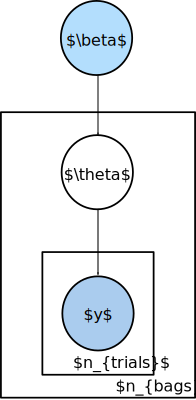
\includegraphics[width=\textwidth]{beta_bernoulli.png}
%
\section{Evaluation}
\subsection{Posterior Model check}
\subsection{Bayes Factor}
\subsection{Cross Validation}

\section{Future Works}

\section{Conclusion}
% ---- Bibliography ----
%
\bibliographystyle{apalike} 
\bibliography{proposal.bib}
\end{document}
